\documentclass[tikz,border=2pt]{standalone}
\usepackage{amsmath,amssymb}
\usepackage{tikz}
\usetikzlibrary{arrows.meta}

\begin{document}
% Local extrema in the plane: a hilltop (local max) and a hollow (local min), each compared
% only with points inside a small neighbourhood U.
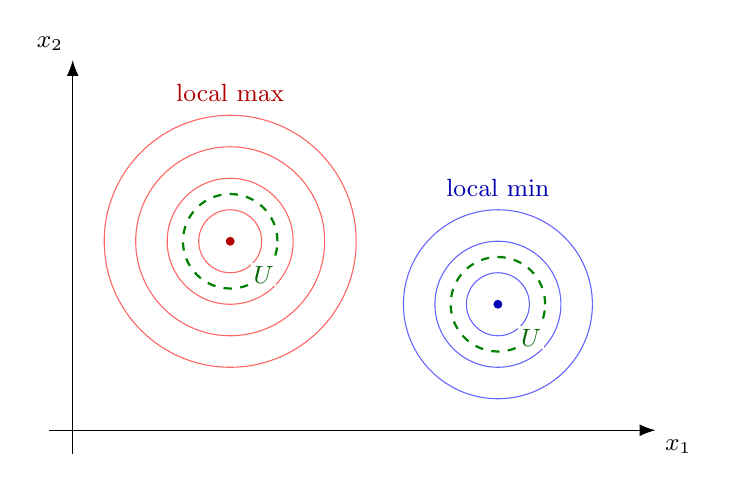
\begin{tikzpicture}[every node/.style={font=\small}, >={Latex[length=2mm]}, lab/.style={font=\small, fill=white, inner sep=1pt}]
	\draw[->] (-0.3,0) -- (7.4,0) node[below right] {$x_1$};
	\draw[->] (0,-0.3) -- (0,4.7) node[above left] {$x_2$};
	\foreach \r in {0.4,0.8,1.2,1.6} {\draw[red!60] (2,2.4) circle (\r);}
	\fill[red!70!black] (2,2.4) circle (1.6pt);
	\node[red!70!black, font=\small, anchor=south] at (2,4.05) {local max};
	\foreach \r in {0.4,0.8,1.2} {\draw[blue!60] (5.4,1.6) circle (\r);}
	\fill[blue!70!black] (5.4,1.6) circle (1.6pt);
	\node[blue!70!black, font=\small, anchor=south] at (5.4,2.85) {local min};
	\draw[green!50!black, thick, dashed] (2,2.4) circle (0.6);
	\node[green!40!black, lab] at (2.424,1.976) {$U$};
	\draw[green!50!black, thick, dashed] (5.4,1.6) circle (0.6);
	\node[green!40!black, lab] at (5.824,1.176) {$U$};
\end{tikzpicture}
\end{document}
